%! TeX program = lualatex
\documentclass[main]{subfiles}

\begin{document}

\title[AutoML: BO]{Bayesian Optimization}
\subtitle{Surrogates, Acquisitions, and Final Best Under Noise}
\author[Bernd Bischl]{Bernd Bischl}
\date{}

\titlebackground*{images/AutoML_HPO_bayesian3.jpg}

    \maketitle


\begin{frame}[t]{Noisy Evaluations}
  \begin{itemize}
    \item So far we assumed noise-free evaluations of $\cost(\conf)$
    \item In practice we only observe a noisy read-out
        $$y = \cost(\conf) + \epsilon, \quad \epsilon \sim \normaldist(0, \noisevar)$$
    \item Sources in HPO: resampling / CV splits, stochastic optimizers, mini-batching, data augmentation
    \item Also outside ML: oil-well estimates, robot-gait measurements, simulator stochasticity
  \end{itemize}
  \vfill
  \begin{center}
    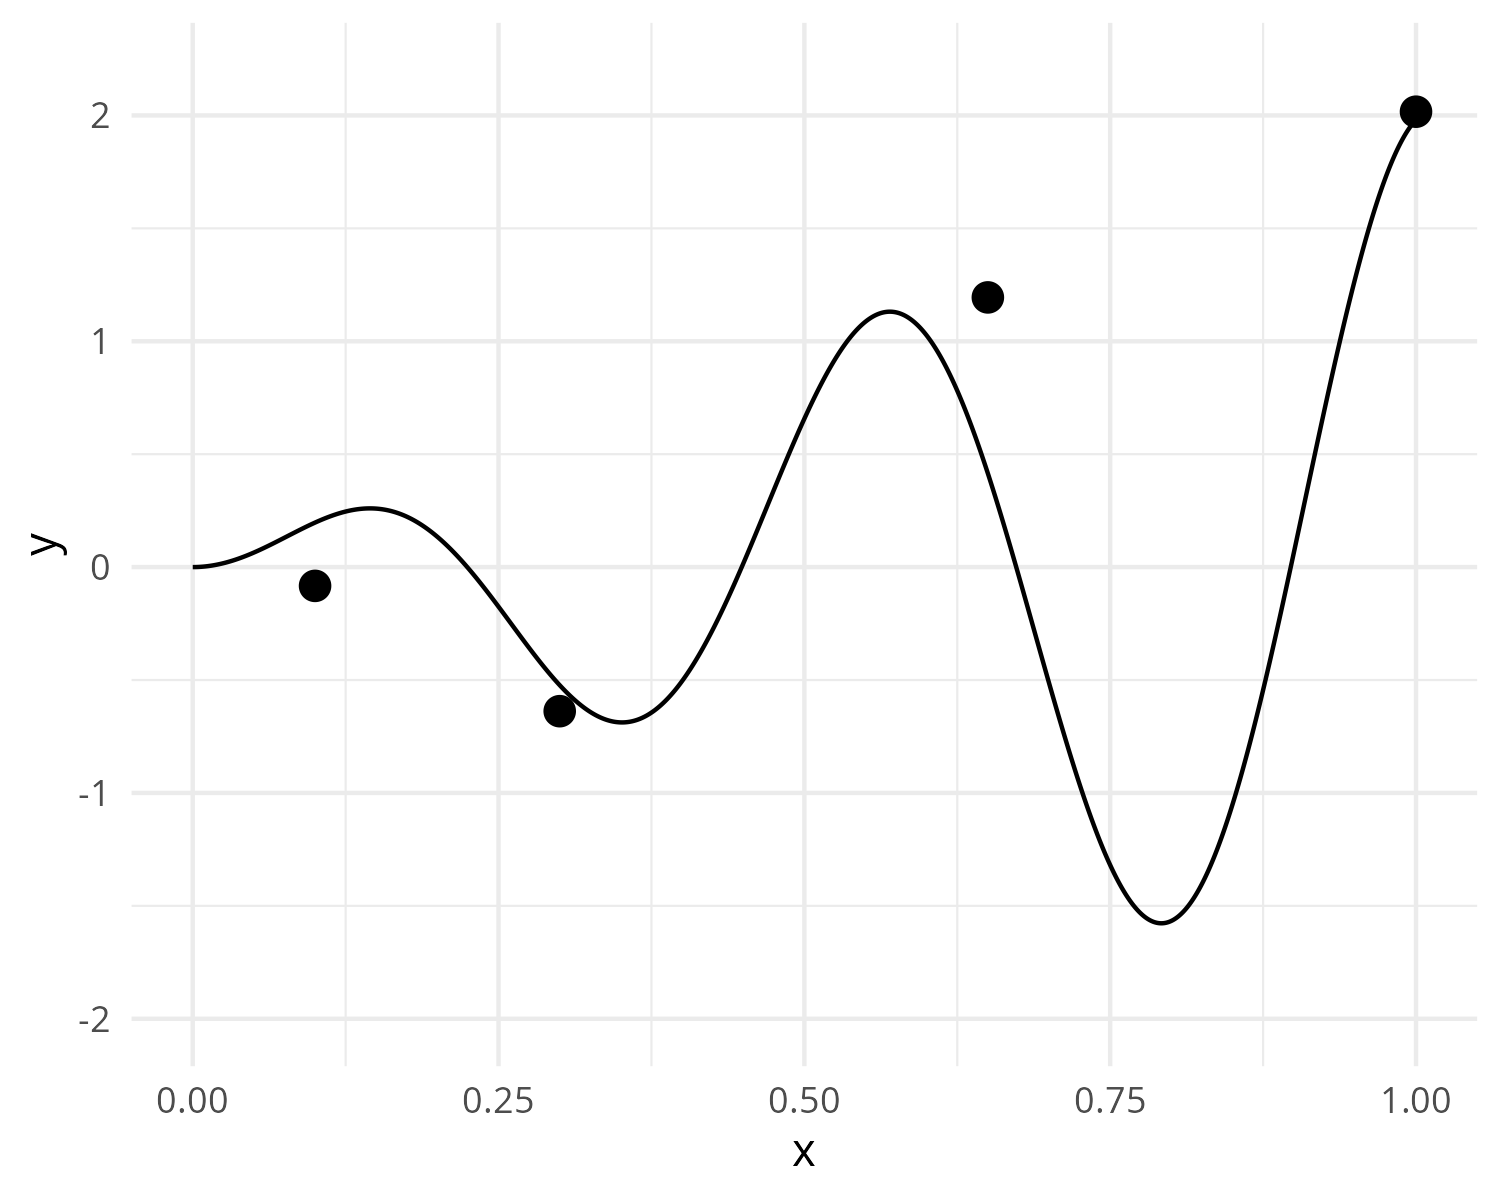
\includegraphics[width=.45\textwidth, height=2.5cm, keepaspectratio]{images/noisy_0.png}
  \end{center}
\end{frame}


\begin{frame}[t]{What Breaks Under Noise?}
  \begin{itemize}
    \item \textbf{Surrogate:} interpolating GP forces $\sh^2(\confI{i}) = 0$ at design points -- wrong, posterior should stay uncertain
    \item \textbf{Acquisition:} PI / EI use $\cmin = \min_i y_i$, but that is a noisy random variable $\leadsto$ lucky outliers dominate
    \item \textbf{Final best point:} the empirically best observation is not the true best -- bad points get overrated by chance, good points overlooked
  \end{itemize}
  \vspace{0.2cm}
  \textbf{Three fixes, one per problem:} noise-aware surrogate, noise-aware ACQF, robust incumbent rule.
\end{frame}


\begin{frame}[t]{Noise-Aware Surrogate: Nugget GP}
  \begin{columns}[onlytextwidth,T]
    \column{.55\textwidth}
    \begin{itemize}
      \item Add nugget $\noisevar \bm{I}$ to the Gram matrix:
        $$\surro(\conf) = k_*^T (\bm{K} + \noisevar \bm{I})^{-1} \yv$$
        $$\sh^2(\conf) = k_{**} - k_*^T (\bm{K} + \noisevar \bm{I})^{-1} k_*$$
      \item Posterior \textbf{smooths} through the data instead of interpolating
      \item $\sh^2(\confI{i}) > 0$ even at design points
      \item $\noisevar$ learned via type-II maximum likelihood alongside the kernel HPs
    \end{itemize}
    \column{.45\textwidth}
    \begin{center}
      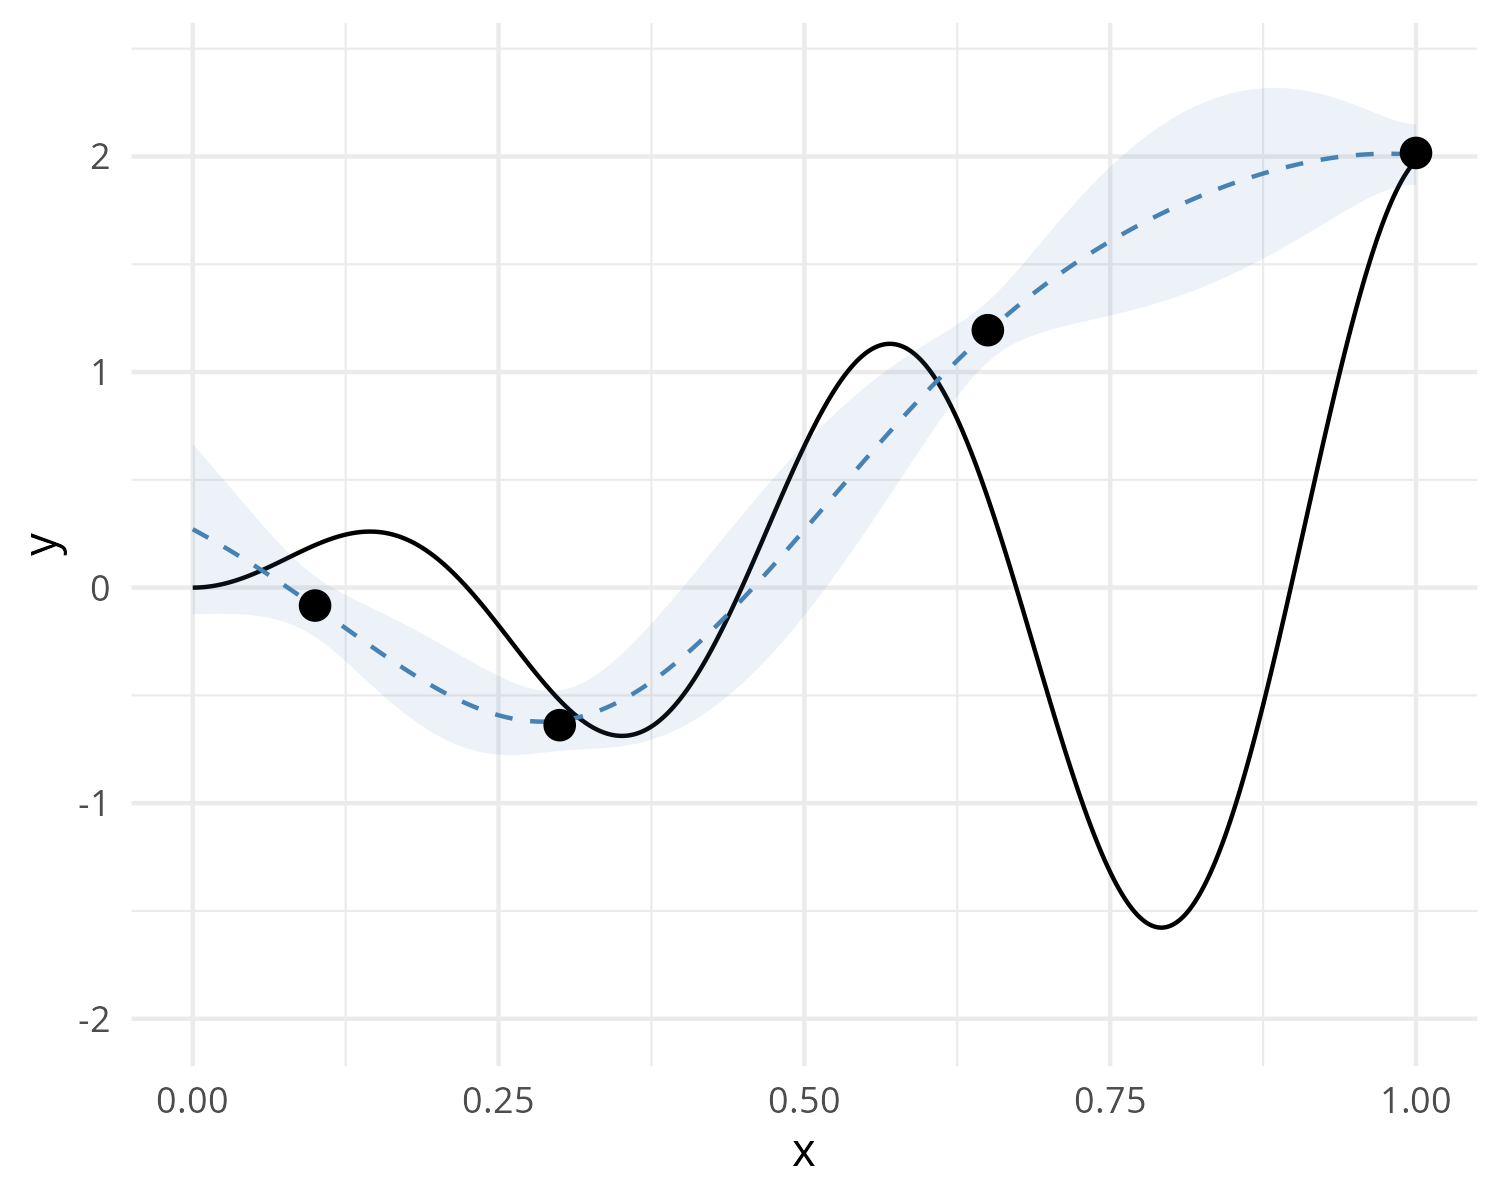
\includegraphics[width=\textwidth]{images/noisy_2.png}
    \end{center}
  \end{columns}
\end{frame}


\begin{frame}[t]{Noise-Aware Acquisition: AEI and NEI}
  \small
  \textbf{Plug-in EI.} Replace unknown $\cmin$ with an \textbf{effective best}:
  $$\cmin^* = \min_{i = 1, \ldots, t} \surro(\confI{i}) + c\, \sh(\confI{i})$$
  Risk-aversion $c \ge 0$ down-weights points with uncertain mean.
  \vspace{0.1cm}
  \begin{itemize}
    \item \textbf{Augmented EI}~\liturl{Huang et al. 2006}{https://link.springer.com/article/10.1007/s10898-005-2454-3}: plug-in EI times a diminishing-returns penalty
      $$\acq_{\text{AEI}}(\conf) = \acq_{\text{EI}_{\cmin^*}}(\conf) \cdot \left(1 - \frac{\sqrt{\noisevar}}{\sqrt{\sh^2(\conf) + \noisevar}}\right)$$
      Penalty shrinks acquisition where the GP is already certain $\leadsto$ redirects budget to replication and exploration. Recovers standard EI as $\noisevar \to 0$.
    \item \textbf{Noisy EI (NEI)}~\liturl{Letham et al. 2019}{https://projecteuclid.org/journals/bayesian-analysis/volume-14/issue-2/Constrained-Bayesian-Optimization-with-Noisy-Experiments/10.1214/18-BA1110.full}: integrate EI over posterior fantasies of the true $(\cost(\confI{i}))$, estimated by MC -- no plug-in needed, plays well with $q$EI / constraints
  \end{itemize}
\end{frame}


\begin{frame}[t]{Which Point to Return?}
  Do \textbf{not} return $\argmin_i y_i$ -- that is the noisy empirical min, prone to lucky outliers.
  \vspace{0.1cm}
  \begin{itemize}
    \item \textbf{Model-based incumbent:} return $\argmin_i \surro(\confI{i})$ -- the design point with the best predicted mean
    \item \textbf{Risk-averse:} $\argmin_i \surro(\confI{i}) + c\, \sh(\confI{i})$ (same as the AEI plug-in) -- punish uncertain candidates
    \item \textbf{Replication strategies:} re-evaluate the current incumbent (and maybe close competitors) to reduce noise on the decisive point
    \item \textbf{Posterior-mean argmin on the whole domain:} $\argmin_{\conf \in \pcs} \surro(\conf)$ -- may fall outside the evaluated history, so only trust if the GP is well-calibrated
  \end{itemize}
  \vfill
  \begin{center}
    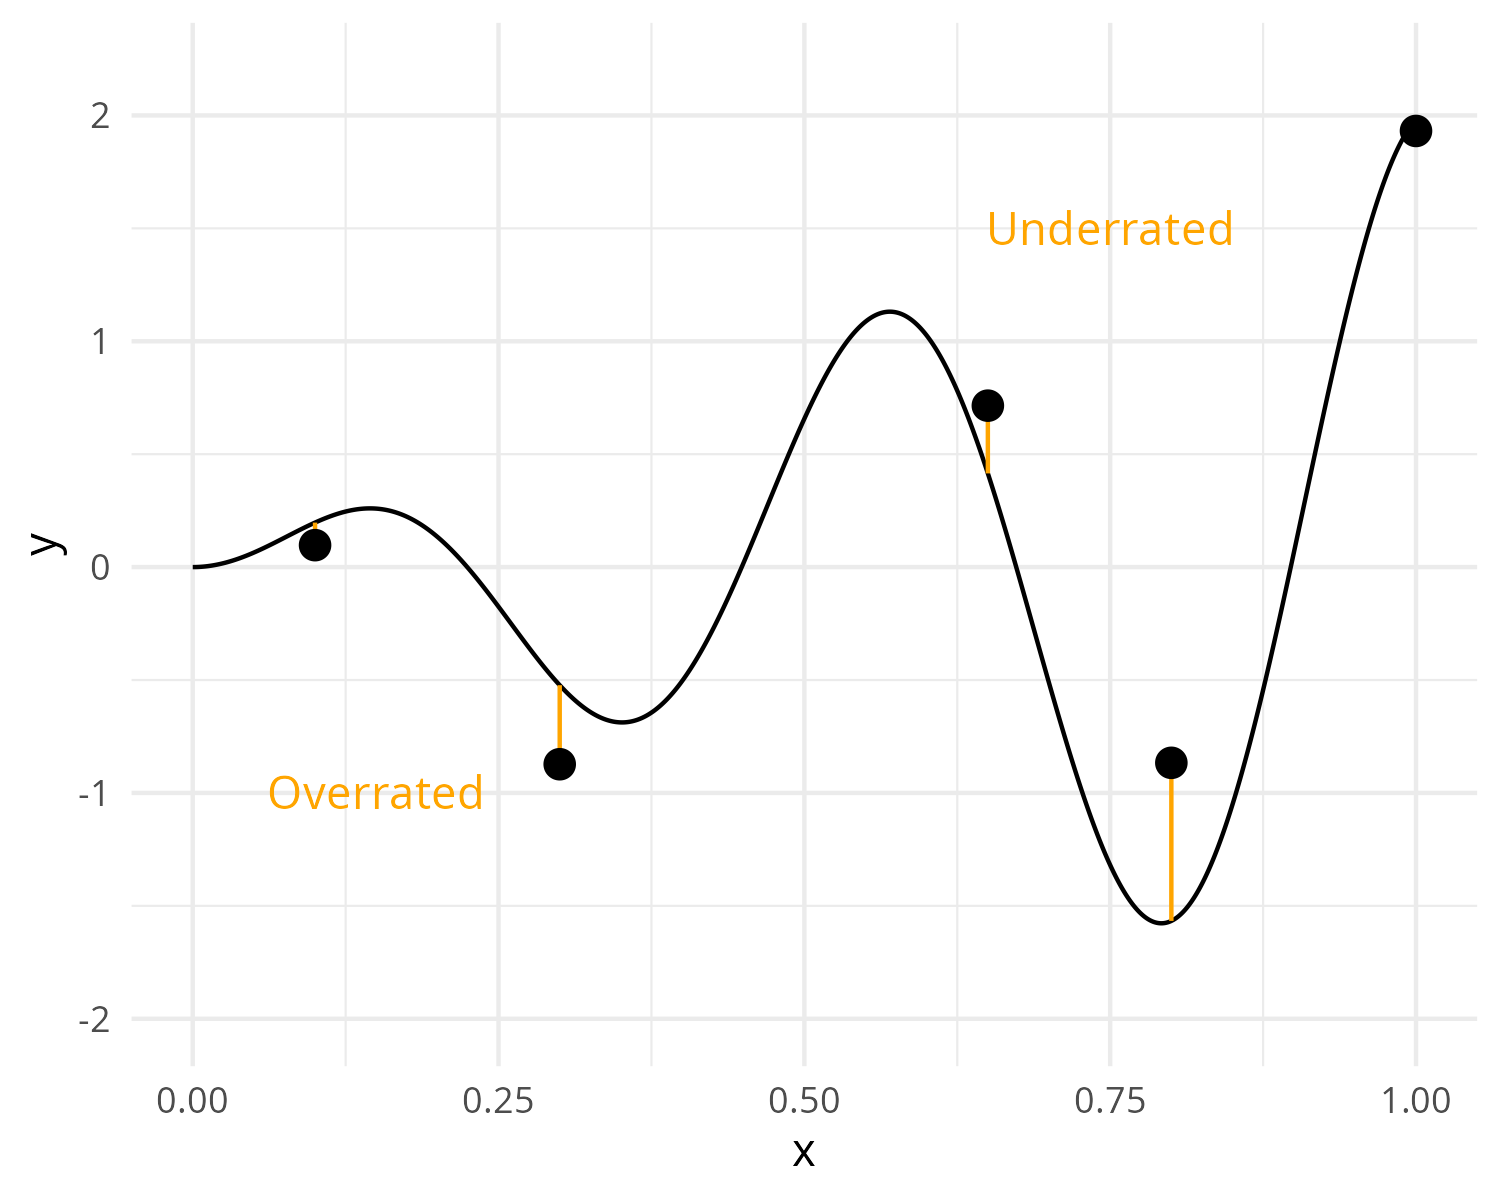
\includegraphics[width=.4\textwidth, height=2.5cm, keepaspectratio]{images/noisy_5.png}
  \end{center}
\end{frame}


\begin{frame}[t]{Summary}
  \begin{enumerate}
    \item Noise breaks three things: interpolating surrogate, $\cmin$-based acquisition function, and empirical best-point identification
    \item \textbf{Surrogate:} switch to a nugget GP (regression mode); learn $\noisevar$ via type-II ML
    \item \textbf{Acquisition:} use a plug-in incumbent $\cmin^*$; AEI adds a diminishing-returns penalty, NEI integrates EI over posterior fantasies
    \item \textbf{Final best:} return the model-based (or risk-averse) incumbent, replicate the current best to sharpen its estimate
    %\item Connects to \textbf{multi-fidelity} BO (not covered here): trade cheap-and-noisy for expensive-and-accurate evaluations
  \end{enumerate}
\end{frame}


\end{document}
